\chapter{Software Implementation}

In order to test the main hypothesis of \say{Does the use of fuzzy entropy alignment metrics improve the alignment of mammograms?} an application was needed to portray the visual output. It would be built to take a set of input images, allow the user to select the alignment metric plus select how many iterations they would like completed and output the final congealed image. Details of the decreasing entropy would be a key output, along with the average image after each iteration completed, for a full picture of improvements.

\section{Implementation Tools}

This section will going into detail about the tools and programming language used to implement the application built to support the hypotheses.

\subsection{Tool \& Programming Language: MATLAB}
\label{ssec:matlab}

MATLAB \cite{MATLAB:2016} was chosen as the main implementation tool and programming language for the project as it is specifically designed to aid in scientific research. Furthermore, MATLAB was the ideal choice as the original \Gls{Congealing} algorithm was implemented in MATLAB. Other alternative languages, as outlined below, were ruled out:

\begin{itemize}
  \item Java: after contacting Learned-Miller directly, it was concluded that there was no \Gls{Congealing} algorithm demo code programmed in Java. The author did not want to further increase the workload to create a Java implementation as this could put the project at risk of non-completion.
  \item C++: the author decided not to pursue using a C++ implementation of the \Gls{Congealing} algorithm, as in the public Git repository by `Debonet' \cite{cpp_congealing}, due to lack of experience in the language.
\end{itemize}

MATLAB offers a lot of built-in packages designed to alleviate the more mundane implementation tasks, such as reading in images (function \texttt{imread}) and applying functions to every item in a matrix (function \texttt{bsxfun}). This also leads to quicker run-times as MATLAB relies heavily on vectorisation of code (as outlined later in the document - Section \ref{sec:tech-diff}), which reduces the time spent running \texttt{for} loops.

However, to use MATLAB as a student, a license must be purchased. This costs \pounds29 + VAT as a stand-alone product, with additional Toolboxes costing an extra \pounds16 each. The open-source alternative Octave \cite{octave} was considered for a while, however due to original code having been developed in MATLAB, porting it over to Octave may have raised technical issues before the project has even begun.

\subsection{Tool: Version Control}

Version control is an important tool in modern day software creation. It records changes to files (such as code or written documents), and allows the user to update versions, or rollback to a previous version. In teams this is vital due to developers often working on the same, or similar, pieces of code simultaneously.

The tools utilised for version control in this project were Git \cite{2014gits}, Github online \cite{github} and Github desktop tool \cite{github_desktop}.

Git \cite{2014gits} is one of the most popular in terms of \acrfull{SCM} tools. It is a command-line tool which allows you to work on sections of code completely independent of each other and later merge them back into one complete article. Due to being written in C, Git is extremely quick compared to its rivals, being up to 325 times faster than \acrfull{SVN} \cite{About_Git}.

Github \cite{github} - \url{github.com} - is an online hosting service for Git repositories. It allows the user to clearly see all the files in the repository, make minor changes via an online editor, and to easily track features such as issues and feature requests. By offering both public and private repositories Github allows developers to work on new, incomplete projects that only they or their team can see, or to open-source their completed software and make it freely available to the world.

Github also allows visualisations of the commit history to the repository, as demonstrated in Figure \ref{fig:git-graph}.

\begin{figure}[H]
  \centering
  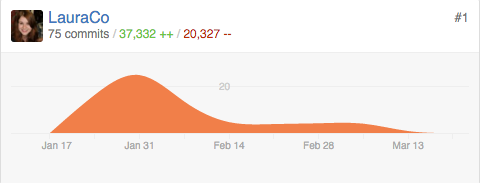
\includegraphics[width=0.6\textwidth]{Chapter2/tools/git_graph.png}
  \caption{Graph outlining git commit history in one branch during the project.}
  \label{fig:git-graph}
\end{figure}

Github desktop \cite{github_desktop} is a simple tool which leverages the power of both Git and Github. It allows the user to run commands usually executed via the command line in a \acrshort{GUI} and provides a graphical representation of the repository being worked in. This reduces the complexity of using branches, as the user can simply compare their current branch against others, and pull, push, merge and create pull requests as desired. Due to it being created by Github, instead of a third party, this ensures that Git is always up to date, and it seemlessly links in with the online project repository.

In order to sustain a solid Git flow each new feature, such as Hybrid entropy implementation or \acrshort{GUI} implementation, was developed in its own branch. Each new feature was branched off of the  main development branch, so the content was always up to date. Once a feature had been completed, changes would be pushed back up to the development branch, ready for the next feature to leverage the functionality.
